% This is the Amherst College LaTeX thesis template.
% See http://web.reed.edu/cis/help/latex.html for help. There are a
% great bunch of help pages there, with notes on
% getting started, bibtex, etc. Go there and read it if you're not
% already familiar with LaTeX.
%
% Any line that starts with a percent symbol is a comment.
% They won't show up in the document, and are useful for notes
% to yourself and explaining commands.
% Commenting also removes a line from the document;
% very handy for troubleshooting problems. -BTS

% As far as I know, this follows the requirements laid out in
% the 2002-2003 Senior Handbook. Ask a librarian to check the
% document before binding. -SN

%%
%% Preamble
%%
% \documentclass{<something>} must begin each LaTeX document
\documentclass[12pt,twoside]{amherstthesis}
% Packages are extensions to the basic LaTeX functions. Whatever you
% want to typeset, there is probably a package out there for it.
% Chemistry (chemtex), screenplays, you name it.
% Check out CTAN to see: http://www.ctan.org/
%%
\usepackage{graphicx,latexsym}
\usepackage{amsmath}
\usepackage{amssymb,amsthm}
\usepackage{longtable,booktabs,setspace}
\usepackage{chemarr} %% Useful for one reaction arrow, useless if you're not a chem major
\usepackage{rotating}

% Modified by CII
\usepackage[hyphens]{url}
\usepackage{hyperref}
\usepackage{lmodern}

% Added by CII (Thanks, Hadley!)
% Use ref for internal links
\renewcommand{\hyperref}[2][???]{\autoref{#1}}
\def\chapterautorefname{Chapter}
\def\sectionautorefname{Section}
\def\subsectionautorefname{Subsection}

\usepackage{caption}
\captionsetup{width=5in}

% \usepackage{times} % other fonts are available like times, bookman, charter, palatino

\title{Exposition of Spatial Clustering Methods}
\author{Kaitlyn E. Haase}
% The month and year that you submit your FINAL draft TO THE LIBRARY (May or December)
\date{February 2019}
\division{Statistics}
\advisor{Advisor A. Wagaman}
%If you have two advisors for some reason, you can use the following
%\altadvisor{Your Other Advisor}
%%% Remember to use the correct department!
\department{Mathematics and Statistics}
% if you're writing a thesis in an interdisciplinary major,
% uncomment the line below and change the text as appropriate.
% check the Senior Handbook if unsure.
%\thedivisionof{The Established Interdisciplinary Committee for}
% if you want the approval page to say "Approved for the Committee",
% uncomment the next line
%\approvedforthe{Committee}

% Below added by CII

%%% Copied from knitr
%% maxwidth is the original width if it's less than linewidth
%% otherwise use linewidth (to make sure the graphics do not exceed the margin)
\makeatletter
\def\maxwidth{ %
  \ifdim\Gin@nat@width>\linewidth
    \linewidth
  \else
    \Gin@nat@width
  \fi
}
\makeatother

\renewcommand{\contentsname}{Table of Contents}

\setlength{\parskip}{0pt}

\providecommand{\tightlist}{%
  \setlength{\itemsep}{0pt}\setlength{\parskip}{0pt}}

\Acknowledgements{
I would like to thank Professor Wagaman for her support through my time
at Amherst. I have enjoyed having her as a professor for three semesters
and advisor. She is an incredibly talented Statistics Professor and has
taught me skills I will be able to take with me beyond my years at
Amherst.
}

\Dedication{

}

\Preface{

}

\Abstract{
In recent years, the amount of geographic data has increased immensely
with new technology (i.e.~GPS and surveillance cameras). Additionally,
the data has improved in accuracy and increased in complexity. This has
provoked statisticians to create techniques to best analyze and draw
conclusions from this new-found data. Earlier techniques of spatial data
were not equipped to handle the complexity and quantity of the data.
This project first explores how and why we analyze data based on
geographic information. Next, I will explain some examples of spatial
data algorithms, including PAM (Partitioning Around Medoids), CLARA
(Clustering LARge Applications), and CLARANS (Clustering Large
Applications based on RANdomized Search). The purpose of this
exploration is to better analyze government health data from a previous
STAT 495 project. I will then: use a sample of STAT 495 project data to
demonstrate the CLARA algorithm, evaluate how CLARA performed, and
develop a model to best predict cluster.
}


%%
%% End Preamble
%%
%

\begin{document}

      \maketitle
  
  \frontmatter % this stuff will be roman-numbered
  \pagestyle{empty} % this removes page numbers from the frontmatter

      \begin{acknowledgements}
      I would like to thank Professor Wagaman for her support through my time
      at Amherst. I have enjoyed having her as a professor for three semesters
      and advisor. She is an incredibly talented Statistics Professor and has
      taught me skills I will be able to take with me beyond my years at
      Amherst.
    \end{acknowledgements}
  
  
  % Add table of abbreviations?

      \hypersetup{linkcolor=black}
    \setcounter{tocdepth}{2}
    \tableofcontents
  
      \listoftables
  
      \listoffigures
  
      \begin{abstract}
      In recent years, the amount of geographic data has increased immensely
      with new technology (i.e.~GPS and surveillance cameras). Additionally,
      the data has improved in accuracy and increased in complexity. This has
      provoked statisticians to create techniques to best analyze and draw
      conclusions from this new-found data. Earlier techniques of spatial data
      were not equipped to handle the complexity and quantity of the data.
      This project first explores how and why we analyze data based on
      geographic information. Next, I will explain some examples of spatial
      data algorithms, including PAM (Partitioning Around Medoids), CLARA
      (Clustering LARge Applications), and CLARANS (Clustering Large
      Applications based on RANdomized Search). The purpose of this
      exploration is to better analyze government health data from a previous
      STAT 495 project. I will then: use a sample of STAT 495 project data to
      demonstrate the CLARA algorithm, evaluate how CLARA performed, and
      develop a model to best predict cluster.
    \end{abstract}
  
  
  \mainmatter % here the regular arabic numbering starts
  \pagestyle{fancyplain} % turns page numbering back on

  \onehalfspacing
  
  \chapter*{Introduction}\label{introduction}
  \addcontentsline{toc}{chapter}{Introduction}
  
  Cassidy Mahar, Silvia Sotolongo, and I, for our STAT 495 project, used
  mapping techniques to visualize and analyze US Government data. The data
  contained spatial, demographic, and health status information. The only
  significant relationships we were able to find were between demographic
  information and health status; we were unable to relate health status
  with any spatial information. I am interested in analyzing the data
  through spatial clustering, to further analyze whether the location of
  an observation is related to one's health status. Since clustering
  utilizes spatial information, it may be helpful in finding patterns in
  the data.
  
  \section{Why Analyze Spatial Data?}\label{why-analyze-spatial-data}
  
  We are interested in analyzing spatial data for many reasons, one being
  because there is so much of it available. Spatial data analysis is
  analyzing data based on topological, geometric, and geographic
  information. Spatial data may include latitude and longitude, zip code,
  or street address. Investigating spatial data can help us find
  dissimilarities and similarities among objects. This can aid in
  allocating resources to areas that need them most, discovering changes
  over time, and categorizing new objects.
  
  \section{Analyzing Spatial Data
  Algorithms}\label{analyzing-spatial-data-algorithms}
  
  Many, many algorithms exist that analyze spatial data; most algorithms
  are focused around clustering. To get a glimpse of the number of
  algorithms and strategies to analyze spatial data, Figure 1 provides
  some examples (Wagaman, 2019).
  
  \begin{figure}[htbp]
  \centering
  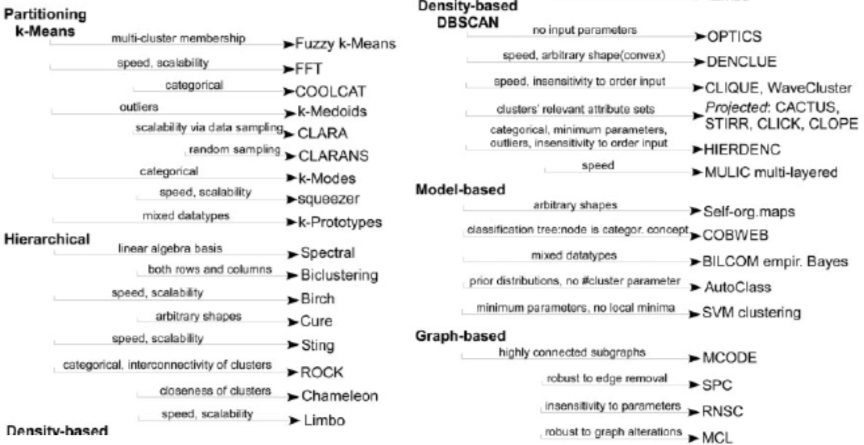
\includegraphics[scale = 0.5,angle = 0]{clustering_methods.png}
  \caption[Clustering Methods]{\normalsize{Clustering Methods}}
  \label{fig:Clustering}
  \end{figure}
  
  As noted, the methods are aimed around clustering, which I will further
  explore in the next section.
  
  \subsection{Clustering}\label{clustering}
  
  Clustering organizes a set of data items into groups so that items in
  the same group are similar to each other and different from those in
  other groups (Huo \& Mennis, 2009). Clustering is helpful in finding
  patterns and similarities/differences between data points and groups;
  however it can be quite subjective. It is up to the statistician to
  determine how many clusters are appropriate for the data, as well as the
  cut off for what is considered ``similar'' or ``dissimilar''.
  Additionally, the statistician must choose which clustering algorithm is
  best to use.
  
  \chapter{Clustering Basics}\label{rmd-basics}
  
  Since there are so many clustering algorithms, choosing the appropriate
  method becomes an important task. There are many factors to consider
  when choosing a clustering algorithm, such as the application of the
  problem (what do you want to find out about this data?), quality versus
  speed trade off (the size of the data plays a role), characteristics of
  the data (i.e.~numeric distance measures), dimensionality (typically as
  dimension increases, the time it takes to run the method increases and
  quality of the data clusters decrease), and outliers (some methods are
  very sensitive to outliers) (Jiawei Han \& Tung, n.d.). These were some
  of the considerations I had to think about in analyzing the data from my
  STAT 495 project.
  
  \section{Partitioning}\label{partitioning}
  
  There are four main types of clustering: hierarchical, partitioning,
  density-based, and methods-based. Next, I'll dive into the partitioning
  clustering technique.
  
  Partitioning cluster methods divide a set of data items into a number of
  non-overlapping clusters. A data item is typically assigned to a cluster
  based on a proximity or dissimilarity measure (Jiawei Han \& Tung,
  n.d.).
  
  Usually, there is a data set with \(n\) observations and the goal is to
  divide the data points into \(k\) clusters so that an objective function
  is optimized.
  
  The most common objective function is the sum of squared errors (SSE),
  where \(c_k\) is the centroid or medoid of the cluster \(C_k\).
  
  \[SSE(C)= \sum_{k=1}^K \sum_{x_{i} in C_{k}} ||{x_i}- c_k||^2\] Note:
  the ``element-of'' symbol would not work in Latex, so I am using ``in''
  to indicate this instead.
  
  Partitioning clustering algorithms classify the data into K groups by
  satisfying both that each group has at least one data point, and that
  each data point belongs to exactly one group (V \& Surendran, 2013).
  
  \section{Methods to Create Clusters}\label{methods-to-create-clusters}
  
  There are many ways to create clusters. The most basic method is the
  \(K\)-means algorithm, which was developed by MacQueen in 1967 (V \&
  Surendran, 2013). In response to \(K\)-means being very sensitive to
  outliers, the \(K\)-medoid algorithm was created in 1987 (V \&
  Surendran, 2013). Both partitioning methods use iterative processes to
  find \(K\) clusters; however, they use different ways to represent these
  clusters.
  
  \subsection{\texorpdfstring{\emph{K}-Means}{K-Means}}\label{k-means}
  
  \(K\)-means algorithm represents its \(n\) observations in \(k\) groups,
  with the center of the groups being the mean/average observation. The
  goal of the algorithm is to find \emph{k} centroids, one for each
  cluster. In order to do this, we must minimize an objective function,
  which is the squared error function for \(k\) means. The objective
  function is: \[O= \sum_{j=1}^k \sum_{i=1}^j ||{{X_i^{(j)}- C_j}}||^2\]
  
  Where \(|{{X_i^{(j)}- C_j}}|\) is an indicator of the distance of the
  data points from their cluster centers.
  
  The steps of the algorithm are as follows (V \& Surendran, 2013):
  
  \begin{enumerate}
  \def\labelenumi{\arabic{enumi}.}
  \item
    Choose \(k\) points in the space to represent the centroids. This
    works best if they are chosen to be far apart from each other.
  \item
    Assign each object in the data set to the cluster with the closest
    centroid.
  \item
    When all of the clusters have been made, recalculate the positions of
    the \(k\) centroids.
  \item
    Repeat steps 2 and 3 until the centroids no longer move.
  \end{enumerate}
  
  This algorithm always terminates; however, it is sensitive both to
  outliers and to the initial randomly selected \emph{k} cluster centers.
  Therefore, the algorithm should be run multiple times to reduce the
  effects from this sensitivity.
  
  In order to determine how well \(K\)-means worked, we use the within
  cluster sum-of-squares, WSS, to determine the compactness/``goodness''
  of the clustering (and we want it as small as possible).
  
  We calculate the WSS by the following equation:
  
  \[WSS = \sum_{k=1}^k \sum_{x_i in C_k} ({{x_i- \mu_k}})^2\] Where
  \(x_i\) is a data point in cluster \(C_k\) and \(\mu_k\) is the mean
  value assigned to the cluster \(C_k\) (Datanovia, n.d.).
  
  \subsection{\texorpdfstring{\emph{K}-Medoids}{K-Medoids}}\label{k-medoids}
  
  On the contrary, instead of taking the mean value of the objects in a
  cluster to be the center, the \(k\)-medoid method uses the most
  centrally located object in a cluster to be the cluster center (Jiawei
  Han \& Tung, n.d.). This causes the method to be less sensitive to
  outliers, but also requires more time to run.
  
  Steps for \(K\)-medoids (V \& Surendran, 2013):
  
  \begin{enumerate}
  \def\labelenumi{\arabic{enumi}.}
  \item
    Initial guess for centers \(C_1\), \(C_2\),\ldots{} \(C_k\)
    (i.e.~randomly select \emph{k} points from \(X_1\), \(X_2\),\ldots{}
    \(X_n\))
  \item
    Minimize over C: for each i= 1, 2,\ldots{} n, find the cluster center
    \(C_k\) closest to Xi and let C(i)=k.
  \item
    Minimize over \(C_1\), \(C_2\),\ldots{} \(C_k\): for each k=1,\ldots{}
    K, \(C_k = X_k^*\), the medoid of points in cluster k. ie, the point
    Xi in the cluster k that minimizes
    \[\sum  _{c(j)=k} ||{{X_j- X_i}}||^2\]
  \end{enumerate}
  
  Basically, \(K\)-means and \(K\)-medoids follow very similar algorithms;
  however, \(K\)-medoids uses the most centrally located object (medoid)
  in a cluster to be the cluster center. This causes there to only be at
  most one center changed for each iteration (makes the algorithm run
  slower).
  
  \section{\texorpdfstring{How to Choose
  \(K\)}{How to Choose K}}\label{how-to-choose-k}
  
  Now that we've discussed \(K\)-means and \(K\)-medoids partitioning
  methods, we know how to find \(k\) clusters of data points; but how do
  we determine what \(k\) is?
  
  Well, there are many ways to choose \(k\), which is why these methods
  are so subjective.
  
  I will describe two of the many ways to determine \(k\), both of which
  use visuals to determine what value of \(k\) is appropriate for the
  data. The elbow method and silhouette method are common ways to find
  \(k\) when using the \(K\)-means and \(K\)-medoids algorithms
  (Datanovia, n.d.).
  
  \subsection{Elbow Method}\label{elbow-method}
  
  To start, the Elbow method looks at the total within-cluster sum of
  squares (WSS) and determines when there are enough clusters so that the
  next cluster does not improve the total WSS very much. This would be the
  appropriate \(k\) to choose.
  
  The steps for this algorithm are as follows (Datanovia, n.d.):
  
  \begin{enumerate}
  \def\labelenumi{\arabic{enumi}.}
  \item
    Compute the clustering algorithm (i.e. \emph{k}-medoids method) for
    different values of \(k\) (i.e. \(k\) from 1 to 10).
  \item
    For each \(k\), calculate the total WSS. WSS can be calculated as:
  \end{enumerate}
  
  \[WSS= \sum_{i=1}^k \sum_{x_i in C_k} ||{{x_i- c_k}}||^2\] Where \(x_i\)
  is a data point in cluster \(C_k\) and \(c_k\) is the medoid assigned to
  the cluster \(C_k\). (Datanovia, n.d.).
  
  \begin{enumerate}
  \def\labelenumi{\arabic{enumi}.}
  \setcounter{enumi}{2}
  \item
    Plot the curve of the total WSSs according to the number of clusters
    (k).
  \item
    The location of the bend in the plot is generally considered an
    indicator for the appropriate number of clusters.
  \end{enumerate}
  
  \subsection{Silhouette Method}\label{silhouette-method}
  
  The Silhouette method focuses on the quality of clustering. A high
  average silhouette width indicates a good clustering (how well each
  object lies within its cluster).
  
  The steps of the Silhouette Algorithm are (Datanovia, n.d.):
  
  \begin{enumerate}
  \def\labelenumi{\arabic{enumi}.}
  \item
    Compute clustering algorithm for different values of \emph{k} (i.e.
    \emph{k} from 1 to 10).
  \item
    For each \emph{k}, calculate the average silhouette of observations.
  \end{enumerate}
  
  The silhouette of an object \(O_j\), is a quantity varying between -1
  and 1, that indicates how much \(O_j\) truly belongs to the cluster to
  which \(O_j\) is classified (Ng \& Han, 2000).
  
  There is a silhouette function in R that calculates the silhouette
  widths of the clusters.
  
  \begin{enumerate}
  \def\labelenumi{\arabic{enumi}.}
  \setcounter{enumi}{2}
  \item
    Plot the curve of the average silhouettes according to the number of
    clusters (k).
  \item
    The location of the maximum is considered the appropriate number of
    clusters.
  \end{enumerate}
  
  \chapter{Clustering Methods Continued}\label{typeset-equ}
  
  \section{PAM}\label{pam}
  
  Partitioning Around Medoids (PAM) is the most commonly used type of
  \(k\)-medoid clustering (Kaufmann \& Rousseeuw, 1987).
  
  As an overview, the algorithm iterates through all the \(k\) cluster
  centers and tries to replace the center with one of the other objects
  (\(n-k\) possibilities) (Jiawei Han \& Tung, 2002). For a replacement to
  occur, the squared error function must decrease. If it does not
  decrease, there is no replacement. The algorithm eventually terminates.
  
  For the set up of this algorithm, let's let \(O_m\) be a current medoid
  that is to be replaced (i.e.~A in Figure 2.1). Let's let \(O_p\) be a
  new medoid to replace \(O_m\) (i.e.~M in Figure 2.1). \(O_j\) is an
  other non-medoid object that may or may not be moved (i.e.~Y and Z in
  Figure 2.1). \(O_{j,2}\) is a current medoid that is nearest to \(O_j\)
  without A and M (i.e.~B in Figure 2.1).
  
  \begin{figure}[htbp]
  \centering
  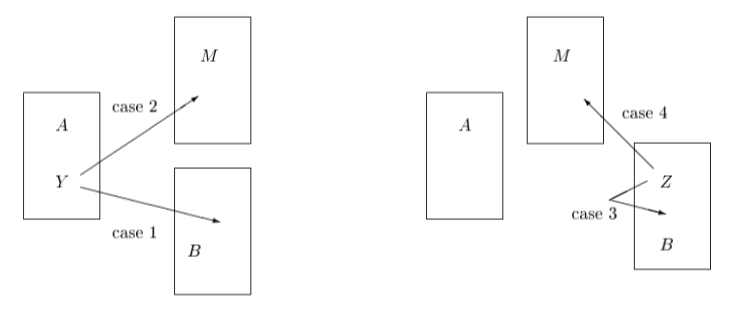
\includegraphics[scale = 0.5,angle = 0]{PAM_pic.png}
  \caption[Four cases for Replacing A with M]{\normalsize{Four cases for Replacing A with M}}
  \label{fig:PAM}
  \end{figure}
  
  Now that I have set us up, there are four different ways or ``cases'' in
  which PAM calculates the cost, \(C_{jmp}\), for all of the non-medoid
  objects \(O_j\) (Jiawei Han \& Tung, n.d.). For the sake of simplicity
  and in understanding the different cases in terms of Figure 2.1, I will
  denote \(O_m\) as A, \(O_p\) as M, \(O_j\) as Y or Z, \(O_{j,2}\) as B.
  
  \textbf{Case 1:}
  
  Suppose Y currently belongs to the cluster represented by A.
  Additionally, Y is more similar to B than to M (i.e.
  \(d(Y, M) \geq d(Y, B)\)), where B is the second most similar medoid to
  Y. If A were to be replaced by M as a medoid, Y would belong to B
  (indicated by the Case 1 arrow in Figure 2.1). Therefore the cost of the
  switch is: \(C_{jmp} = d(Y, B) - d(Y, A)\).
  
  This equation will always give a non-negative \(C_{jmp}\), indicating
  that there is a non-negative cost incurred in replacing A with M.
  
  \textbf{Case 2:}
  
  Suppose Y currently belongs to the cluster represented by A. But this
  time, A is less similar to B than to M (\(d(Y, M) < d(Y, B)\)). Then, if
  A is replaced by M, Y would belong to the cluster represented by M. The
  cost of this swap would be: \(C_{jmp} = d(Y, M) - d(Y, A)\). The value
  of this \(C_{jmp}\) could be positive or negative, depending on whether
  Y is more similar to A or M.
  
  \textbf{Case 3:}
  
  Suppose Z currently belongs to the cluster other than the one
  represented by A. Also, let Z be more similar to B than to M. Then even
  if A is replaced by M, Z would stay in the cluster represented by B. The
  cost of this swap is: \(C_{jmp} = 0\).
  
  \textbf{Case 4:}
  
  Suppose Z belongs to a cluster represented by B, but Z is less similar
  to B than to M. If we replaced A with M, Z would jump to the cluster of
  M, from that of B. The cost in this case would be:
  \(C_{jmp} = d(Z, M) - d(Z, B)\). This cost would always be negative.
  
  In combining all of the four cases described, the total cost of
  replacing A with M is: \[ TC_{mp} = \sum_j(C_{jmp}) \].
  
  The more formal steps of the algorithm are (Jiawei Han \& Tung, n.d.):
  
  \begin{enumerate}
  \def\labelenumi{\arabic{enumi}.}
  \item
    Select \emph{k} representative objects arbitrarily.
  \item
    Compute \(TC_{mp}\) for all pairs of \(O_m\), \(O_p\) where \(O_m\) is
    currently selected, and \(O_p\) is not.
  \item
    Select the pair \(O_m\), \(O_p\) which corresponds to
    \(min_{O_m, O_p} TC_{mp}\). If the minimum \(TC_{mp}\) is negative,
    replace \(O_m\) with \(O_p\) and go back to Step 2.
  \item
    Otherwise, for each non-selected object, find the most similar
    representative object.
  \end{enumerate}
  
  The total complexity of PAM in one iteration is \(O(k(n-k)^2)\) (O= each
  non-medoid data point, \emph{k}= \# of cluster centers, \((n-k)\)
  objects to compare to, and \((n-k)\) operations for calculating E). This
  makes for a costly computation when \emph{n} is large. The algorithm
  works best when \emph{n}= 100 and \emph{k}=5.
  
  \section{CLARA}\label{clara}
  
  Because PAM does not scale well to large data sets, Clustering LARge
  Applications (CLARA) was developed (Kaufmann \& Rousseeuw, 1990).
  
  CLARA is a sampling based method, meaning a sample of the data is used
  to represent the entire data set. Medoids are chosen from this sample
  data using PAM and then the average dissimilarity is computed using the
  whole data set, not only the objects in the samples. If a new set of
  medoids gives a lower dissimilarity than a previous best solution, then
  the best solution is replaced with a new set of medoids (Jiawei Han \&
  Tung, n.d.).
  
  Experiments indicate that 5 samples of size 40+ 2\(k\) give satisfactory
  results (Ng \& Han, 2000).
  
  The steps for the algorithm are as follows (Jiawei Han \& Tung, n.d.):
  
  \begin{enumerate}
  \def\labelenumi{\arabic{enumi}.}
  \item
    For i= 1 to 5, repeat the following steps:
  \item
    Draw a sample of 40+ 2\(k\) objects from the entire data set, and use
    PAM to find \emph{k} medoids of the sample.
  \item
    For each object \(O_j\) in the entire data set, determine which of the
    \emph{k} medoids are most similar to \(O_j\).
  \item
    Calculate the average dissimilarity of the clustering obtained in the
    previous step. If this value is less than the current minimum, use
    this value as the current minimum, and retain the \emph{k} medoids
    found in Step 2 as the best medoids obtained so far.
  \item
    Return to Step 1 to start the next iteration.
  \end{enumerate}
  
  CLARA performs well on large data sets, i.e.~around 1000 objects
  (\emph{n}) in 10 clusters (\emph{k}). CLARA can work on larger data sets
  because the complexity for each iteration is
  \(O{k(40 + k)^2 + k(n-k)}\), which is much smaller than \(O(k(n-k)^2)\)
  (which is the complexity for each iteration in PAM) (J. Han, n.d.).
  
  \section{CLARANS}\label{clarans}
  
  CLARANS was created to handle even larger data sets than CLARA, and
  provides the highest quality clusters, in comparison to PAM and CLARA.
  
  The easiest way to understand CLARANS, is through a graphic example
  involving both PAM and CLARA as well (Jiawei Han \& Tung, n.d.).
  
  The processes of finding \emph{k} medoids can be described as searching
  through a graph of objects. This graph, denoted \(G_{n,k}\) contains
  nodes represented by a set of \emph{k} objects
  \{\(O_{m1},... , O_{mk}\)\}, indicating that the medoids of the objects
  are: \(O_{m1},... , O_{mk}\). The set of nodes in the graph is the set
  \{\{\(O_{m1},... , O_{mk}\)\} \textbar{} \(O_{m1},... , O_{mk}\) are
  objects in the data set\}.
  
  Two nodes are considered neighbors if their sets differ by only one
  object. Furthermore, two nodes, \(S_1\) = \{\(O_{m1},... , O_{mk}\)\}
  and \(S_2\) = \{\(O_{w1},... , O_{wk}\)\} are neighbors if the
  intersection of \(S_1, S_2\) is \emph{k}-1. Each node therefore has
  \(k(n-k)\) neighbors. Each node is a cluster; each node can be assigned
  a cost that defines the total dissimilarity between every object and the
  medoid of its cluster.
  
  PAM can be viewed as a search for a minimum on the graph \(G_{n,k}\). At
  each iteration, the neighbors of the current node are examined, and the
  current node gets replaced by the neighbor with the greatest descent in
  costs. The search continues until a minimum is obtained. Examining
  \(k(n-k)\) neighbors of a node is time consuming, which is why CLARA was
  created.
  
  CLARA examines fewer neighbors and restricts the search in general on
  subgraphs of \(G_{n,k}\). The subgraph, \(G_{Sa,k}\), contains all the
  nodes that are subgraphs of \(Sa\). CLARA searches through the nodes
  using PAM, however, the search is confined within \(G_{Sa,k}\). This is
  problematic, because if M is the minimum node in the original graph
  \(G_{n,k}\), but if M is not included in \(G_{Sa,k}\), M will never be
  found. To make up for this deficiency, many, many samples would have to
  be collected and processed (Jiawei Han \& Tung, 2002).
  
  CLARANS was developed because of this deficiency. CLARANS does not
  restrict to a particular subgraph, instead it searches the entire graph
  \(G_{n,k}\). CLARANS is unlike PAM in that it only checks a subgroup of
  the neighbors of a node (like CLARA). But in contrast to CLARA, each
  sample is drawn in a way that no nodes corresponding to particular
  objects are outright eliminated.
  
  CLARA draws a sample of \emph{nodes} at the beginning of the search,
  while CLARANS draws a sample of \emph{neighbors} in each step of a
  search. CLARANS provides higher quality clusters than CLARA and only
  requires few searches.
  
  For the CLARANS algorithm, there are two parameters used:
  \emph{maxneighbor} (the maximum numbers of neighbors examined) and
  \emph{numlocal} (the number of local minima obtained). The higher the
  value of maxneighbor, the closer CLARANS is to PAM.
  
  Steps for the CLARANS algorithm (Jiawei Han \& Tung, 2002):
  
  \begin{enumerate}
  \def\labelenumi{\arabic{enumi}.}
  \tightlist
  \item
    Input parameters \emph{maxneighbor} and \emph{numlocal}. Initialize i
    to 1, and mincost to a large number.
  \item
    Set \emph{current} to an arbitrary node in \(G_{n,k}\).
  \item
    Set \emph{j}=1.
  \item
    Consider a random neighbor of \emph{S} of \emph{current}. Calculate
    the cost differential of the two nodes, using:
    \[ TC_{mp} = \sum_j(C_{jmp}) \]
  \item
    If \emph{S} has a lower cost, set \emph{current} to \emph{S}, and go
    to Step 3.
  \item
    Otherwise, increment \emph{j} by 1. If \(j \leq maxneighbor\), go to
    Step 4.
  \item
    Otherwise, when \(j > maxneighbor\), compare the cost of \(current\)
    compared to \(mincost\). If \(current < mincost\), set \(mincost\) to
    the cost of \(current\), and set \(bestnode\) to \(current\).
  \item
    Increment \emph{i} by 1. If \(i > numlocal\), output \(bestnode\) and
    stop. Otherwise, go to Step 2.
  \end{enumerate}
  
  Since my data from my STAT 495 project has over 60,000 observations, I
  originally wanted to apply the CLARANS method. Unfortunately, the
  CLARANS function in R only works for SNP data (used in biology).
  Therefore, I had to take a representative sample my data, and apply the
  CLARA method instead.
  
  \chapter{Application to Health Data}\label{typeset-equ}
  
  \section{Exploring the Data}\label{exploring-the-data}
  
  In this application, I will further explore the data from my STAT 495
  final project. The data is from DataUSA, which uses public US Government
  data to analyze and visualize relationships (DataUSA, n.d.). In the
  previous project, we decided to use data from only 2016 because of size
  restrictions. The data contains spatial information, quantitative
  variables, and a few categorical variables.
  
  The data contains demographic information, latitude and longitude, and
  variables that are indicators of health status. The health status
  variables include: poor to fair health (the percentage of adults
  reporting fair or poor health (age-adjusted)), poor physical health days
  (average number of physically unhealthy days reported in the past 30
  days (age-adjusted)), physical inactivity (the percentage of adults aged
  20 and over reporting no leisure-time physical inactivity), and adult
  obesity (the percentage of adults to report a BMI of greater than or
  equal to 30). In interpreting the health indicator variables, the higher
  the values for these variables, the less healthy a person is.
  
  My research question is to see whether there are clusters of people with
  exceptionally good or exceptionally poor health. This information could
  lead to further insights into what environmental or other factors are
  impacting peoples' health.
  
  I plan to use the CLARA method, since I have more than 100 observations
  (PAM works on data sets of \(n\)=100). The data set has over 60,000
  observations, so I will need to sample about 1000 observations in order
  to produce the best results using CLARA.
  
  I will first take a random sample of 1000 observations. I assume the
  sample is representative of the data set because \emph{n} is so large
  (\emph{n} = 1000).
  
  \begin{Shaded}
  \begin{Highlighting}[]
  \KeywordTok{set.seed}\NormalTok{(}\DecValTok{1}\NormalTok{)}
  \CommentTok{#getting a sample of 1000 observations}
  \NormalTok{mysample <-}\StringTok{ }\NormalTok{data_subset[}\KeywordTok{sample}\NormalTok{(}\DecValTok{1}\OperatorTok{:}\KeywordTok{nrow}\NormalTok{(data_subset), }\DecValTok{1000}\NormalTok{,}
     \DataTypeTok{replace=}\OtherTok{FALSE}\NormalTok{),]}
  \end{Highlighting}
  \end{Shaded}
  
  The data set I imported has 64 variables, which are too many for this
  example. Since my research question is focused around peoples' health, I
  will include four health indicator variables and the latitude and
  longitude of the data (spatial information).
  
  \begin{Shaded}
  \begin{Highlighting}[]
  \CommentTok{#only keeping the variables I want to look at}
  \NormalTok{myvars <-}\StringTok{ }\KeywordTok{c}\NormalTok{(}\StringTok{"Latitude_tri"}\NormalTok{, }\StringTok{"Longitude_tri"}\NormalTok{, }\StringTok{"poor_or_fair_health"}\NormalTok{, }
              \StringTok{"poor_physical_health_days"}\NormalTok{, }\StringTok{"physical_inactivity"}\NormalTok{, }\StringTok{"adult_obesity"}\NormalTok{)}
  \NormalTok{smallsample <-}\StringTok{ }\NormalTok{mysample[myvars]}
  \NormalTok{new<-}\StringTok{ }\KeywordTok{na.omit}\NormalTok{(smallsample) }\CommentTok{#getting rid of missing data}
  \end{Highlighting}
  \end{Shaded}
  
  The data is now ready for the application of CLARA.
  
  \section{Applying CLARA}\label{applying-clara}
  
  \textbf{Step 1}: Determining \(k\).
  
  One of the important steps in clustering algorithms is determining how
  many \(k\) clusters are appropriate. In Chapter 1, I explained the Elbow
  and Silhouette methods to determine \(k\). I will perform both methods
  on this data to start.
  
  \begin{Shaded}
  \begin{Highlighting}[]
  \CommentTok{#finding k using Elbow Method}
  \KeywordTok{fviz_nbclust}\NormalTok{(new, kmeans, }\DataTypeTok{method =} \StringTok{"wss"}\NormalTok{) }\OperatorTok{+}
  \StringTok{    }\KeywordTok{geom_vline}\NormalTok{(}\DataTypeTok{xintercept =} \DecValTok{4}\NormalTok{, }\DataTypeTok{linetype =} \DecValTok{2}\NormalTok{)}\OperatorTok{+}
  \StringTok{  }\KeywordTok{labs}\NormalTok{(}\DataTypeTok{subtitle =} \StringTok{"Elbow method"}\NormalTok{)}
  \end{Highlighting}
  \end{Shaded}
  
  \begin{center}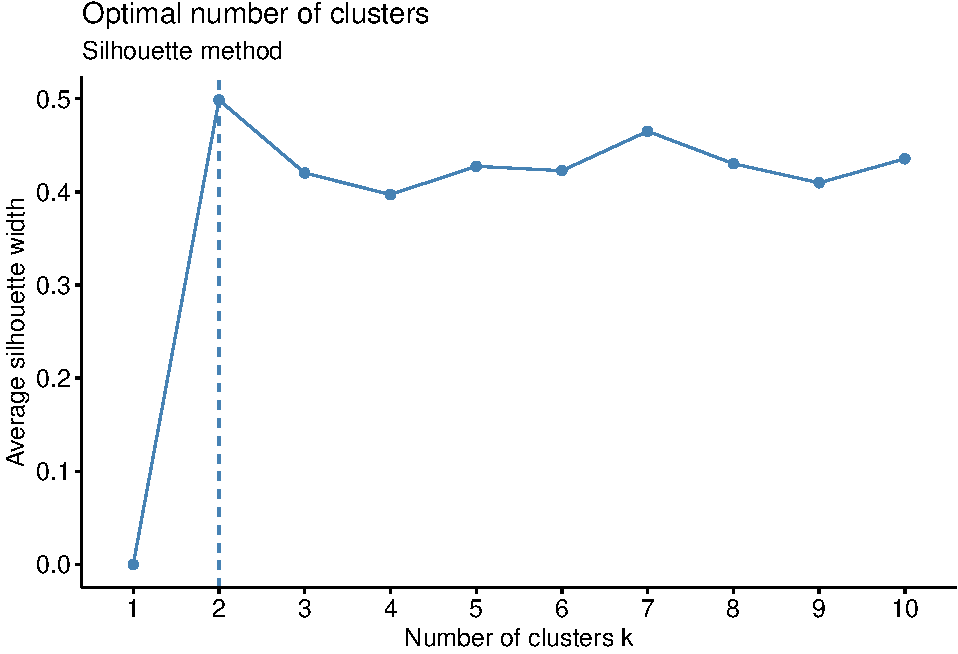
\includegraphics{Comps_Proj_files/figure-latex/unnamed-chunk-5-1} \end{center}
  
  \begin{Shaded}
  \begin{Highlighting}[]
  \KeywordTok{fviz_nbclust}\NormalTok{(new, kmeans, }\DataTypeTok{method =} \StringTok{"silhouette"}\NormalTok{) }\OperatorTok{+}
  \StringTok{  }\KeywordTok{labs}\NormalTok{(}\DataTypeTok{subtitle =} \StringTok{"Silhouette method"}\NormalTok{)}
  \end{Highlighting}
  \end{Shaded}
  
  \begin{center}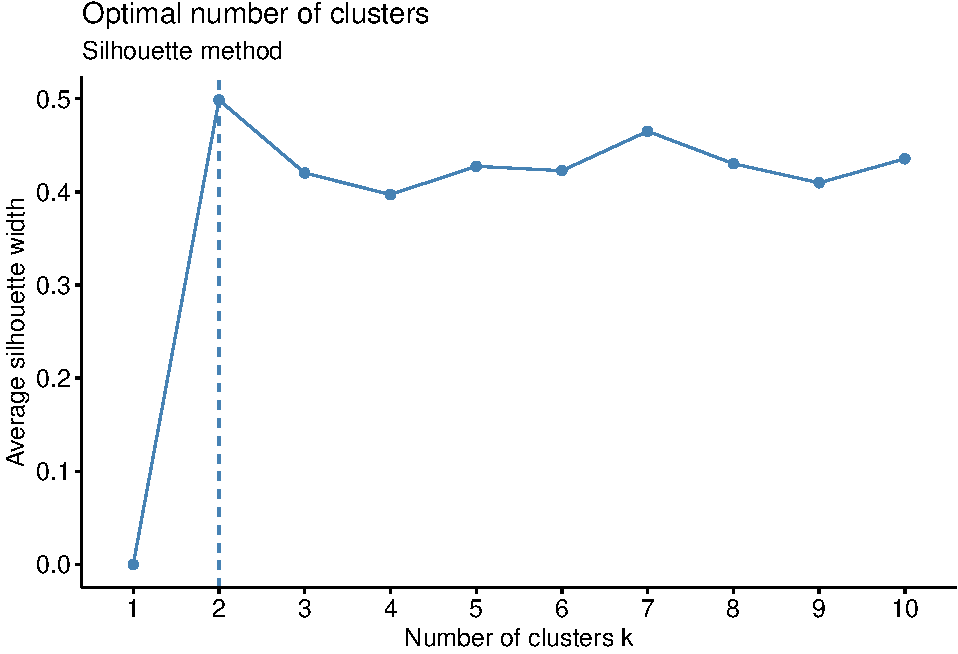
\includegraphics{Comps_Proj_files/figure-latex/unnamed-chunk-5-2} \end{center}
  
  According to the Elbow method, \(k\) should be 4 (where the elbow is in
  the graph). According to the Silhouette method, \(k\) should be 2 (the
  maximum point in the graph). Since there is variation in values of \(k\)
  for these methods I will take the average of the two to determine \(k\).
  
  \textbf{Step 2}: Run CLARA function
  
  Next, I will run the CLARA algorithm on the data, using the criteria of
  \(k\)=3.
  
  \begin{Shaded}
  \begin{Highlighting}[]
  \NormalTok{## run CLARA}
  \NormalTok{clarasamp <-}\StringTok{ }\KeywordTok{clara}\NormalTok{(new[}\DecValTok{1}\OperatorTok{:}\DecValTok{6}\NormalTok{], }\DecValTok{3}\NormalTok{)}
  \end{Highlighting}
  \end{Shaded}
  
  \begin{Shaded}
  \begin{Highlighting}[]
  \NormalTok{## print components of clara}
  \KeywordTok{print}\NormalTok{(clarasamp)}
  \end{Highlighting}
  \end{Shaded}
  
  \begin{verbatim}
  Call:    clara(x = new[1:6], k = 3) 
  Medoids:
       Latitude_tri Longitude_tri poor_or_fair_health
  [1,]      39.3265      -84.4388               0.155
  [2,]      40.3973      -75.9357               0.165
  [3,]      36.1336      -96.1039               0.196
       poor_physical_health_days physical_inactivity adult_obesity
  [1,]                       3.7               0.232         0.289
  [2,]                       3.7               0.245         0.308
  [3,]                       4.6               0.353         0.355
  Objective function:  5.659219
  Clustering vector:   int [1:925] 1 2 1 3 1 3 1 1 1 1 1 3 1 2 1 3 1 3 ...
  Cluster sizes:           457 205 263 
  Best sample:
   [1]   5  24  86 139 149 175 177 192 208 224 242 285 306 316 333 353 361
  [18] 370 389 400 404 410 429 468 471 489 502 506 567 593 679 691 703 719
  [35] 726 741 780 800 811 815 818 877 882 883 902 918
  
  Available components:
   [1] "sample"     "medoids"    "i.med"      "clustering" "objective" 
   [6] "clusinfo"   "diss"       "call"       "silinfo"    "data"      
  \end{verbatim}
  
  This output tells us a lot about the results of the clustering. To
  start, the information from the Medoids section show that cluster 3
  contains people with the worst health, in comparison to cluster 1 and 2.
  For example, cluster 1 and 2 average 3.7
  \emph{poor\_physical\_health\_days}, while cluster 3 averages 4.6. This
  difference was seen in all four health indicator variables.
  
  The cluster sizes are also noted. There are 457 observations in cluster
  1, 205 in cluster 2, and 263 in cluster 3.
  
  \begin{Shaded}
  \begin{Highlighting}[]
  \CommentTok{#cluster number for each observation}
  \NormalTok{clarasamp}\OperatorTok{$}\NormalTok{cluster}
  \CommentTok{#silhouette width for each cluster}
  \NormalTok{clarasamp}\OperatorTok{$}\NormalTok{silinfo}
  \end{Highlighting}
  \end{Shaded}
  
  This information tells us even more about the CLARA output. The first
  part gives us the categorizations of each data point to its cluster. The
  second part of information gives us the average silhouette width for
  each cluster. The silhouette widths were: 0.422183 for cluster 1,
  0.634548 for cluster 2, and 0.172013 for cluster 3. The better the
  clustering is, the greater the silhouette width; so we can determine
  that cluster 2 was best compared to cluster 1 and 3.
  
  Next, I will walk through some of the visualizations given this new
  clustering information.
  
  \begin{Shaded}
  \begin{Highlighting}[]
  \NormalTok{## plot clusters}
  \KeywordTok{plot}\NormalTok{(new, }\DataTypeTok{col =}\NormalTok{ clarasamp}\OperatorTok{$}\NormalTok{cluster)}
  \NormalTok{## plot centers}
  \KeywordTok{points}\NormalTok{(clarasamp}\OperatorTok{$}\NormalTok{centers, }\DataTypeTok{col =} \DecValTok{1}\OperatorTok{:}\DecValTok{2}\NormalTok{, }\DataTypeTok{pch =} \DecValTok{8}\NormalTok{)}
  \end{Highlighting}
  \end{Shaded}
  
  \begin{center}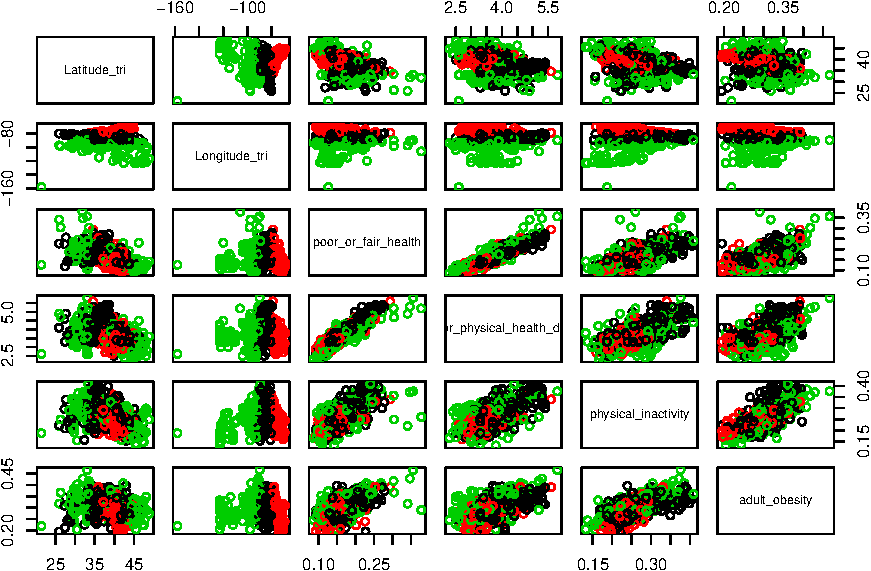
\includegraphics{Comps_Proj_files/figure-latex/unnamed-chunk-9-1} \end{center}
  
  The plot of the clusters does not look great. Aside from comparing
  longitude with the other variables, the plots have entirely overlapping
  clusters. This indicates that the CLARA method was unable to find great
  patterns in the data.
  
  Next, I will use a version of a ggplot to plot the clusters.
  
  \begin{Shaded}
  \begin{Highlighting}[]
  \CommentTok{#plotting clara}
  \NormalTok{factoextra}\OperatorTok{::}\KeywordTok{fviz_cluster}\NormalTok{(clarasamp)}
  \end{Highlighting}
  \end{Shaded}
  
  \begin{center}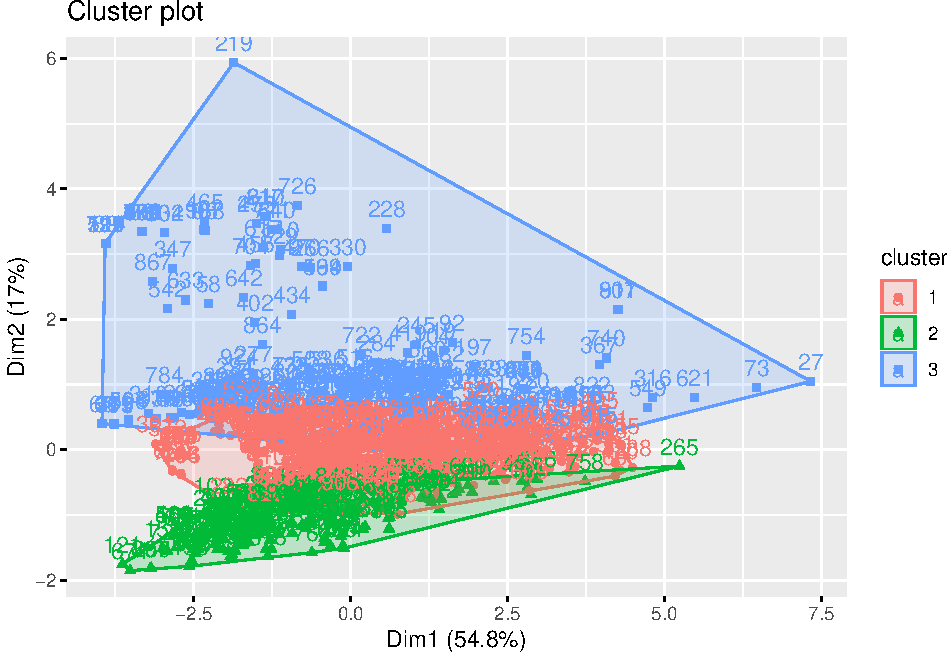
\includegraphics{Comps_Proj_files/figure-latex/unnamed-chunk-10-1} \end{center}
  
  This plot shows the overlapping of the clusters as well.
  
  \section{Evaluation of CLARA}\label{evaluation-of-clara}
  
  There are multiple ways to determine the effectiveness of CLARA and the
  quality of its clusters. One way to internally validate the method, is
  to look at its within-cluster sum of squares (WSS). If the WSS is high,
  it is likely the method did not work very well.
  
  I plotted in the previous section in the Elbow method plot to determine
  the number of clusters to use. Since I decided to use \(k\)=3 clusters,
  I can now go back and calculate the WSS for the method.
  
  \begin{Shaded}
  \begin{Highlighting}[]
  \KeywordTok{fviz_nbclust}\NormalTok{(new, kmeans, }\DataTypeTok{method =} \StringTok{"wss"}\NormalTok{) }\OperatorTok{+}
  \StringTok{    }\KeywordTok{geom_vline}\NormalTok{(}\DataTypeTok{xintercept =} \DecValTok{3}\NormalTok{, }\DataTypeTok{linetype =} \DecValTok{2}\NormalTok{)}\OperatorTok{+}
  \StringTok{  }\KeywordTok{labs}\NormalTok{(}\DataTypeTok{subtitle =} \StringTok{"Elbow method"}\NormalTok{)}
  \end{Highlighting}
  \end{Shaded}
  
  \begin{center}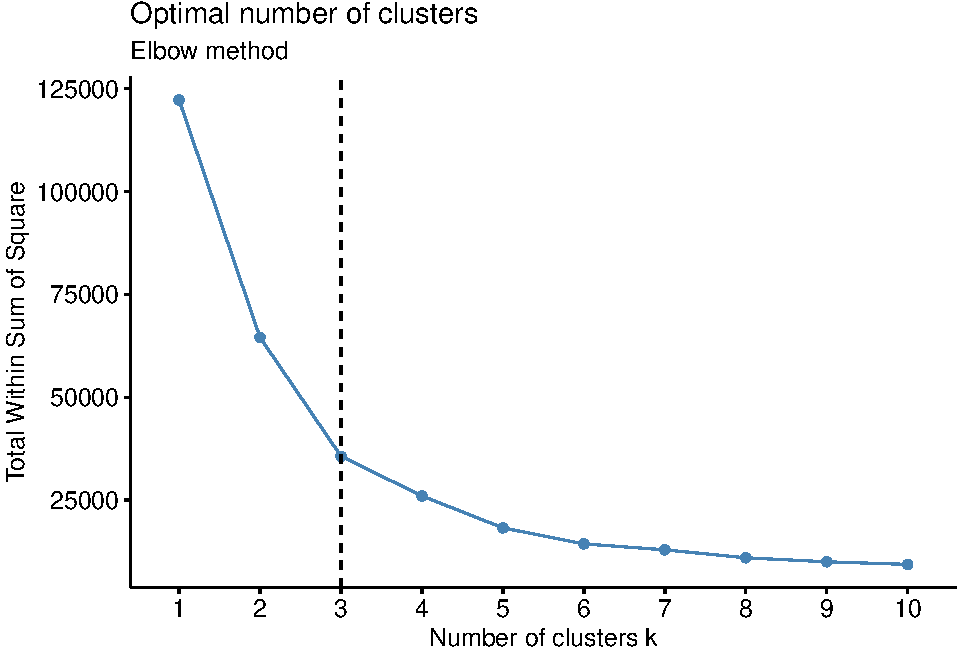
\includegraphics{Comps_Proj_files/figure-latex/unnamed-chunk-11-1} \end{center}
  
  The Elbow method when \(k\)=3, shows a WSS to be about 35,000. This is
  very high, which is a concern when interpreting the cluster results.
  
  Another method is to look at the silhouette widths of the clusters. As
  mentioned in Chapter 1, the Silhouette method helps us determine how
  many clusters best fits the data. The Silhouette widths of the clusters
  determine how well an object truly belongs to its assigned cluster.
  
  Based on many experiments and research, a silhouette width of 0.71-1
  indicates a strong cluster, 0.51-0.7 indicates a reasonable cluster,
  0.26-0.5 indicates a weak or artificial cluster, and less than or equal
  to 0.25 indicates no cluster found (Ng \& Han, 2000).
  
  In this example, the silhouette widths were: 0.422183 for cluster 1,
  0.634548 for cluster 2, and 0.172013 for cluster 3. In analyzing these
  values based on the criteria, cluster 1 is a weak or artificial cluster,
  cluster 2 is a reasonable cluster, and cluster 3 indicates no cluster
  found.
  
  The overall evaluation of CLARA with this data is that the algorithm did
  not work well. The clusters were very weak, therefore, one should not
  draw conclusions based on the results from this analysis.
  
  \subsection{Model to Predict Cluster}\label{model-to-predict-cluster}
  
  The CLARA method found three clusters to group the health data. While
  the WSS value and silhouette widths of the clusters indicated the
  clustering may not be very accurate or useful, I still want to
  investigate if I can predict the cluster number (1, 2, or 3), given the
  health indicator variables. This would be helpful information, if I
  wanted to categorize a new observation, given its values for the health
  variables used.
  
  To start this process, I first had to include a variable with cluster
  number (from the CLARA method) to the original sample of the data set.
  
  \begin{Shaded}
  \begin{Highlighting}[]
  \CommentTok{#adding each data point's cluster #}
  \NormalTok{cluster<-}\StringTok{ }\NormalTok{clarasamp}\OperatorTok{$}\NormalTok{clustering}
  \NormalTok{cluster_data<-}\StringTok{ }\KeywordTok{cbind}\NormalTok{(new, cluster)}
  \end{Highlighting}
  \end{Shaded}
  
  Next, I looked at possible relationships between the health indicator
  variables and cluster number. To start, I quickly looked at a
  multivariate linear regression model to predict cluster using all of the
  possible variables.
  
  \begin{Shaded}
  \begin{Highlighting}[]
  \NormalTok{kitchen_sink<-}\StringTok{ }\KeywordTok{lm}\NormalTok{(cluster}\OperatorTok{~}\NormalTok{., }\DataTypeTok{data=}\NormalTok{cluster_data)}
  \CommentTok{#summary(kitchen_sink)}
  \end{Highlighting}
  \end{Shaded}
  
  \begin{table}[ht]
  \centering
  \begin{tabular}{rrrrr}
    \hline
   & Estimate & Std. Error & t value & Pr($>$$|$t$|$) \\ 
    \hline
  (Intercept) & 0.3835 & 0.3762 & 1.02 & 0.3082 \\ 
    Latitude\_tri & -0.0073 & 0.0065 & -1.12 & 0.2614 \\ 
    Longitude\_tri & -0.0393 & 0.0022 & -17.91 & 0.0000 \\ 
    poor\_or\_fair\_health & 10.0890 & 1.4178 & 7.12 & 0.0000 \\ 
    poor\_physical\_health\_days & -1.0820 & 0.0884 & -12.25 & 0.0000 \\ 
    physical\_inactivity & 1.9868 & 0.7307 & 2.72 & 0.0067 \\ 
    adult\_obesity & 0.3328 & 0.8160 & 0.41 & 0.6835 \\ 
     \hline
  \end{tabular}
  \caption{Kitchen Sink Model} 
  \end{table}
  
  According to this model, \emph{longitude},
  \emph{poor\_or\_fair\_health}, \emph{poor\_physical\_health\_days}, and
  \emph{physical\_inactivity} were strong predictors of cluster number.
  Overall, the model seemed to fit the data fairly well. The model had a
  high F-statistic and a low p-value of \textless{}2e-16. The adjusted
  R-squared value was 0.372.
  
  In analyzing this model I realized that latitude and longitude were used
  as quantitative variables instead of categorical. Since multivariate
  regression predictive models do not use spatial information, I realized
  that the latitude and longitude would not be helpful.
  
  \begin{Shaded}
  \begin{Highlighting}[]
  \CommentTok{#taking out latitude and longitude}
  \NormalTok{vars <-}\StringTok{ }\KeywordTok{names}\NormalTok{(cluster_data) }\OperatorTok\StringTok{ }\KeywordTok{c}\NormalTok{(}\StringTok{"Latitude_tri"}\NormalTok{, }\StringTok{"Longitude_tri"}\NormalTok{)}
  \NormalTok{cluster_data_new <-}\StringTok{ }\NormalTok{cluster_data[}\OperatorTok{!}\NormalTok{vars]}
  \end{Highlighting}
  \end{Shaded}
  
  I ran another full multivariate regression model, an updated kitchen
  sink model, with only the health variables and cluster information.
  
  \begin{Shaded}
  \begin{Highlighting}[]
  \NormalTok{new_kitchen_sink<-}\StringTok{ }\KeywordTok{lm}\NormalTok{(cluster}\OperatorTok{~}\NormalTok{., }\DataTypeTok{data=}\NormalTok{cluster_data_new)}
  \CommentTok{#summary(new_kitchen_sink)}
  \end{Highlighting}
  \end{Shaded}
  
  \begin{table}[ht]
  \centering
  \begin{tabular}{rrrrr}
    \hline
   & Estimate & Std. Error & t value & Pr($>$$|$t$|$) \\ 
    \hline
  (Intercept) & 3.5366 & 0.2297 & 15.40 & 0.0000 \\ 
    poor\_or\_fair\_health & 13.0696 & 1.3988 & 9.34 & 0.0000 \\ 
    poor\_physical\_health\_days & -1.2089 & 0.0964 & -12.54 & 0.0000 \\ 
    physical\_inactivity & -0.9774 & 0.8086 & -1.21 & 0.2270 \\ 
    adult\_obesity & 2.8044 & 0.9247 & 3.03 & 0.0025 \\ 
     \hline
  \end{tabular}
  \caption{Updated Kitchen Sink Model} 
  \end{table}
  
  This model had three significant predictors
  (\emph{poor\_or\_fair\_health}, \emph{poor\_physical\_health\_days}, and
  \emph{adult\_obesity}), a high F-statistic, and a low p-value of
  \textless{}2e-16. The model did not fit the data very well, and had an
  adjusted R-squared value of 0.155.
  
  Next, I looked at the possible correlations between cluster number and
  the health indicator variables. I predicted the healthier people (lower
  scores on the health indicator variables) would be in cluster 1, while
  the least healthy people (higher scores on health indicator variables)
  would be in cluster 3. I also predicted the health indicator variables
  would be highly correlated with each other, considering they all are
  aiding in predicting one's health. My predictions were based on the
  CLARA output from the previous section.
  
  \begin{Shaded}
  \begin{Highlighting}[]
  \KeywordTok{ggpairs}\NormalTok{(cluster_data_new)}
  \end{Highlighting}
  \end{Shaded}
  
  \begin{center}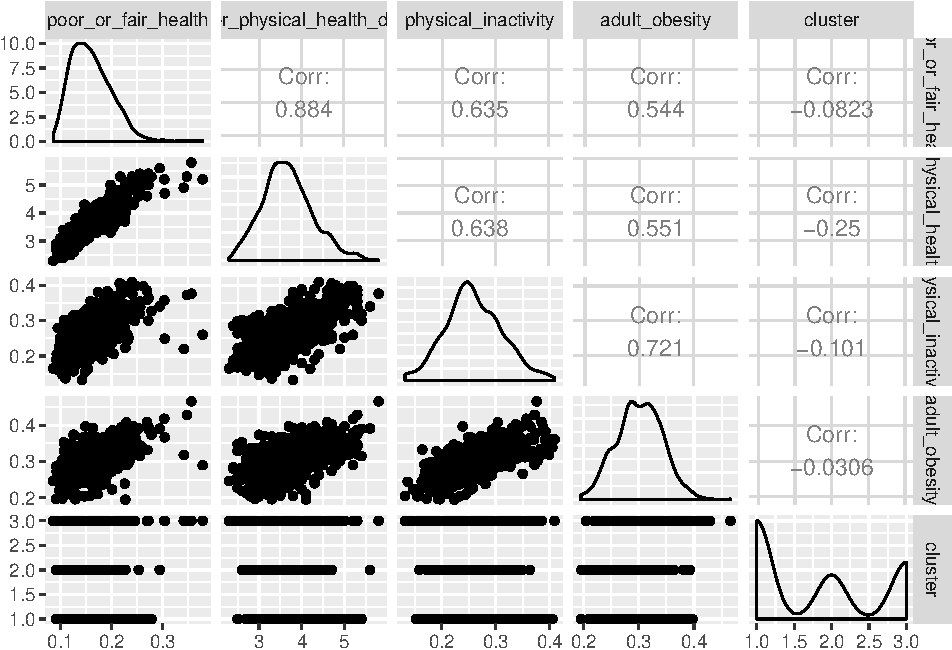
\includegraphics{Comps_Proj_files/figure-latex/unnamed-chunk-18-1} \end{center}
  
  The correlation matrix shows strong positive correlations between
  \emph{poor\_or\_fair\_health}, \emph{poor\_physical\_health\_days},
  \emph{physical\_inactivity}, and \emph{adult\_obesity}, as I had
  predicted. The highest correlation was 0.884, between
  \emph{poor\_physical\_health\_days} and \emph{poor\_to\_fair\_health}.
  All of the variables in general show bell-shaped curves with a
  relatively even shape.
  
  The plots comparing the variables to the cluster number are hard to
  interpret at first. To start, the \emph{poor\_to\_fair\_health} versus
  cluster plot shows that the highest values of
  \emph{poor\_or\_fair\_health} are in cluster 3. These look to be
  possible outliers, but regardless, it confirms the prediction that the
  unhealthy people (high health variable scores) are in cluster 3.
  
  The \emph{poor\_physical\_health\_days} versus cluster number and
  \emph{adult\_obesity} versus cluster number show a couple of
  observations with high health variable scores in cluster 3 as well.
  Again, it is unclear if these points are outliers or not.
  
  In general, the plots show that cluster 2 has the smallest range of
  health scores, which further confirms that cluster 2 had the highest
  quality of clustering (the largest silhouette width). In terms of
  correlation values, cluster number was shows to be sightly negatively
  correlated with \emph{poor\_physical\_health\_days}, with a correlation
  value of -0.25.
  
  I had predicted the correlation to be positive, because the CLARA output
  revealed cluster 3 to have the most unhealthy people. This would mean
  the higher the health variable value, the higher the cluster number.
  Since the correlations are in fact slightly negative, I believe the
  reason for the higher health value mean score from the CLARA output for
  cluster 3 was probably due to the outliers (shown in the plots).
  
  All of correlations between the health variables and cluster number were
  negative, indicating there may be outliers impacting the original
  analysis of CLARA.
  
  Nevertheless, I will continue to explore possible relationships between
  health variables and cluster number. Based on the correlation plot, I
  will explore \emph{poor\_or\_fair\_health} (because of the plot),
  \emph{poor\_physical\_health\_days} (because of the correlation value),
  and \emph{adult\_obesity} (because of the plot).
  
  I tried numerous combinations of the variables as well as interaction
  terms, because the variables are so highly correlated. Some examples of
  the combinations I tried are found in Appendix A.
  
  Most of the models had significant predictors; however, the R-squared
  values were small; indicating that the models did not fit the data very
  well.
  
  In comparing adjusted R-squared values and the number of predictors
  used, the best model ended up being:
  
  \begin{Shaded}
  \begin{Highlighting}[]
  \KeywordTok{summary}\NormalTok{(best_model)}
  \end{Highlighting}
  \end{Shaded}
  
  \begin{table}[ht]
  \centering
  \begin{tabular}{rrrrr}
    \hline
   & Estimate & Std. Error & t value & Pr($>$$|$t$|$) \\ 
    \hline
  (Intercept) & 5.7368 & 0.3607 & 15.90 & 0.0000 \\ 
    poor\_physical\_health\_days & -1.2465 & 0.0895 & -13.92 & 0.0000 \\ 
    adult\_obesity & -4.8119 & 1.0719 & -4.49 & 0.0000 \\ 
    adult\_obesity:poor\_or\_fair\_health & 42.1592 & 4.0394 & 10.44 & 0.0000 \\ 
     \hline
  \end{tabular}
  \caption{Best Model to Predict Cluster} 
  \end{table}
  
  This model uses three predictors and has an R-squared value of 0.1736.
  The model has a high F-statistic and a low p-value of \textless{}2e-16.
  Ultimately, I chose this model because it has the highest R-squared
  value in comparison to the other models tested.
  
  \chapter*{Conclusion}\label{conclusion}
  \addcontentsline{toc}{chapter}{Conclusion}
  
  \setcounter{chapter}{4} \setcounter{section}{0}
  
  In conclusion, clustering methods are very useful for spatial data in
  determining patterns and in visualizing data sets. There are MANY
  algorithms out there that analyze spatial data, and these methods
  continue to grow year to year both in quantity and quality (handling
  more data and higher complexity data). The methods discussed in this
  paper are considered partitioning clustering methods. The most popular
  partitioning clustering method is \emph{K}-means, which was discussed in
  comparison to \emph{K}-medoids. To further dive into \emph{K}-medoids
  algorithms, PAM (Partitioning Around Medoids), CLARA (Clustering LArge
  Applications), and CLARANS (Clustering Large Applications based on
  RANdomized Search) were explored. This fulfilled my first proposed task:
  Exposition of spatial clustering methods (describing and explaining),
  why they are useful, what they tell us, general information, exposition
  of PAM, CLARA, and CLARANS method.
  
  Data from my STAT 495 project provided an explicit example of the CLARA
  algorithm. In my STAT 495 project, we were unable to draw conclusions
  about the health status and location of data observations through
  mapping visualizations. This lead to my interest in further analyzing
  the data using clustering algorithms, such as CLARA.
  
  For the application, the Elbow and Silhouette methods were used to
  determine \emph{k} clusters, and the CLARA algorithm then divided the
  objects into clusters. A brief evaluation of the clusters revealed a
  very high within-cluster sum of squares and low silhouette widths,
  indicating that the clusters were not of great quality. This section
  completed my second proposed task: Perform a CLARA analysis on my data
  or another data set.
  
  In determining whether one could predict an observation's cluster based
  on a person's health status, multivariate linear regression models were
  performed. None of the models proved to be very useful; however, the
  best model ended up being able to predict 17.4\% of the variation in the
  model. The data again didn't seem to have many patterns, which further
  confirmed the results from my STAT 495 project. This completed the third
  and final item on my proposed task list: Perform a model where the
  cluster is the response variable to determine if we can predict the
  cluster of an observation based on other variables in the data.
  
  \appendix
  
  \singlespacing
  
  \chapter{The First Appendix}\label{the-first-appendix}
  
  This first appendix includes all of the R chunks of code that were
  hidden throughout the document.
  
  \subsubsection{In Chapter 1:}\label{in-chapter-1}
  
  \begin{Shaded}
  \begin{Highlighting}[]
  \ControlFlowTok{if}\NormalTok{(}\OperatorTok{!}\KeywordTok{require}\NormalTok{(devtools))}
    \KeywordTok{install.packages}\NormalTok{(}\StringTok{"devtools"}\NormalTok{, }\DataTypeTok{repos =} \StringTok{"http://cran.rstudio.com"}\NormalTok{)}
  \ControlFlowTok{if}\NormalTok{(}\OperatorTok{!}\KeywordTok{require}\NormalTok{(dplyr))}
      \KeywordTok{install.packages}\NormalTok{(}\StringTok{"dplyr"}\NormalTok{, }\DataTypeTok{repos =} \StringTok{"http://cran.rstudio.com"}\NormalTok{)}
  \ControlFlowTok{if}\NormalTok{(}\OperatorTok{!}\KeywordTok{require}\NormalTok{(ggplot2))}
      \KeywordTok{install.packages}\NormalTok{(}\StringTok{"ggplot2"}\NormalTok{, }\DataTypeTok{repos =} \StringTok{"http://cran.rstudio.com"}\NormalTok{)}
  \ControlFlowTok{if}\NormalTok{(}\OperatorTok{!}\KeywordTok{require}\NormalTok{(acstats))\{}
    \KeywordTok{library}\NormalTok{(devtools)}
  \NormalTok{  devtools}\OperatorTok{::}\KeywordTok{install_github}\NormalTok{(}\StringTok{"Amherst-Statistics/acstats"}\NormalTok{)}
  \NormalTok{\}}
  \end{Highlighting}
  \end{Shaded}
  
  \subsubsection{In Chapter 3:}\label{in-chapter-3}
  
  \begin{Shaded}
  \begin{Highlighting}[]
  \CommentTok{#loading in packages}
  \KeywordTok{library}\NormalTok{(readr)}
  \KeywordTok{library}\NormalTok{(factoextra)}
  \KeywordTok{library}\NormalTok{(NbClust)}
  \KeywordTok{library}\NormalTok{(ggplot2)}
  \KeywordTok{library}\NormalTok{(cluster)}
  \KeywordTok{library}\NormalTok{(GGally)}
  \KeywordTok{library}\NormalTok{(knitr)}
  \KeywordTok{library}\NormalTok{(xtable)}
  \KeywordTok{options}\NormalTok{(}\DataTypeTok{xtable.comment=}\OtherTok{FALSE}\NormalTok{)}
  \end{Highlighting}
  \end{Shaded}
  
  \begin{Shaded}
  \begin{Highlighting}[]
  \CommentTok{#using data from final stat 495 project}
  \NormalTok{data_subset <-}\StringTok{ }\KeywordTok{read_csv}\NormalTok{(}\StringTok{"CopyOfdata_subset.csv"}\NormalTok{)}
  \end{Highlighting}
  \end{Shaded}
  
  \begin{Shaded}
  \begin{Highlighting}[]
  \KeywordTok{set.seed}\NormalTok{(}\DecValTok{2}\NormalTok{)}
  \CommentTok{#exploring possible relationships between health variables and cluster number}
  
  \NormalTok{fun1<-}\StringTok{ }\KeywordTok{lm}\NormalTok{(cluster}\OperatorTok{~}\StringTok{ }\NormalTok{poor_or_fair_health }\OperatorTok{+}\StringTok{ }\NormalTok{poor_physical_health_days }\OperatorTok{+}\StringTok{ }\NormalTok{adult_obesity, }\DataTypeTok{data=}\NormalTok{ cluster_data_new)}
  \CommentTok{#low adjusted R-squared (0.155), but significant predictors}
   
  \NormalTok{fun2<-}\StringTok{ }\KeywordTok{lm}\NormalTok{(cluster}\OperatorTok{~}\StringTok{ }\NormalTok{poor_or_fair_health, }\DataTypeTok{data=}\NormalTok{ cluster_data_new)}
  \NormalTok{fun3<-}\StringTok{ }\KeywordTok{lm}\NormalTok{(cluster}\OperatorTok{~}\StringTok{ }\NormalTok{poor_physical_health_days, }\DataTypeTok{data=}\NormalTok{ cluster_data_new)}
  \NormalTok{fun4<-}\StringTok{ }\KeywordTok{lm}\NormalTok{(cluster}\OperatorTok{~}\StringTok{ }\NormalTok{adult_obesity, }\DataTypeTok{data=}\NormalTok{ cluster_data_new)}
  \CommentTok{#low adjusted R-squared, highest of the 3 functions was 0.06}
  
  \NormalTok{fun5<-}\StringTok{ }\KeywordTok{lm}\NormalTok{(cluster}\OperatorTok{~}\StringTok{ }\NormalTok{poor_or_fair_health }\OperatorTok{+}\StringTok{ }\NormalTok{poor_physical_health_days }\OperatorTok{+}\StringTok{ }\NormalTok{adult_obesity }\OperatorTok{+}
  \StringTok{            }\NormalTok{poor_or_fair_health}\OperatorTok{:}\NormalTok{poor_physical_health_days, }\DataTypeTok{data=}\NormalTok{ cluster_data_new)}
  \CommentTok{#added an interaction, raised the adjusted R-squared to 0.165}
  
  \NormalTok{fun6<-}\StringTok{ }\KeywordTok{lm}\NormalTok{(cluster}\OperatorTok{~}\StringTok{ }\NormalTok{poor_or_fair_health }\OperatorTok{+}\StringTok{ }\NormalTok{poor_physical_health_days }\OperatorTok{+}\StringTok{ }\NormalTok{adult_obesity }\OperatorTok{+}
  \StringTok{            }\NormalTok{poor_physical_health_days}\OperatorTok{:}\NormalTok{adult_obesity, }\DataTypeTok{data=}\NormalTok{ cluster_data_new)}
  \CommentTok{#tried a different interaction, about the same adjusted R-squared}
  
  \NormalTok{fun7<-}\StringTok{ }\KeywordTok{lm}\NormalTok{(cluster}\OperatorTok{~}\StringTok{ }\NormalTok{poor_or_fair_health }\OperatorTok{+}\StringTok{ }\NormalTok{poor_physical_health_days }\OperatorTok{+}\StringTok{ }\NormalTok{adult_obesity }\OperatorTok{+}
  \StringTok{            }\NormalTok{poor_or_fair_health}\OperatorTok{:}\NormalTok{adult_obesity, }\DataTypeTok{data=}\NormalTok{ cluster_data_new)}
  \CommentTok{#last combination of an interaction, highest adjusted R-squared yet (0.175)!}
  \CommentTok{#only predictor not significant was poor_or_fair_health}
  
  \NormalTok{best_model<-}\StringTok{ }\KeywordTok{lm}\NormalTok{(cluster}\OperatorTok{~}\StringTok{  }\NormalTok{poor_physical_health_days }\OperatorTok{+}\StringTok{ }\NormalTok{adult_obesity }\OperatorTok{+}
  \StringTok{                  }\NormalTok{poor_or_fair_health}\OperatorTok{:}\NormalTok{adult_obesity, }\DataTypeTok{data=}\NormalTok{ cluster_data_new)}
  \CommentTok{#dropped poor_or_fair_health, about the same adjusted R-squared (0.174)}
  
  \NormalTok{fun9<-}\StringTok{ }\KeywordTok{lm}\NormalTok{(cluster}\OperatorTok{~}\StringTok{ }\NormalTok{poor_physical_health_days }\OperatorTok{+}\StringTok{ }\NormalTok{adult_obesity }\OperatorTok{+}
  \StringTok{            }\NormalTok{poor_physical_health_days}\OperatorTok{:}\NormalTok{adult_obesity, }\DataTypeTok{data=}\NormalTok{ cluster_data_new)}
  \CommentTok{#tried a different interaction, low adjusted R-squared (0.0958)}
  
  \NormalTok{fun10<-}\StringTok{ }\KeywordTok{lm}\NormalTok{(cluster}\OperatorTok{~}\StringTok{ }\NormalTok{poor_physical_health_days }\OperatorTok{+}\StringTok{ }\NormalTok{adult_obesity }\OperatorTok{+}
  \StringTok{             }\NormalTok{poor_or_fair_health}\OperatorTok{:}\NormalTok{poor_physical_health_days, }\DataTypeTok{data=}\NormalTok{ cluster_data_new)}
  \CommentTok{#tried last combination of interaction, adjusted R-squared= 0.166}
  \end{Highlighting}
  \end{Shaded}
  
  \backmatter
  
  \chapter{References}\label{references}
  
  \noindent
  
  \setlength{\parindent}{-0.20in} \setlength{\leftskip}{0.20in}
  \setlength{\parskip}{8pt}
  
  \hypertarget{refs}{}
  \hypertarget{ref-Rec7}{}
  Datanovia. (n.d.). Determining the optimal number of clusters: 3 must
  know methods. Retrieved from
  \url{https://www.datanovia.com/en/lessons/determining-the-optimal-number-of-clusters-3-must-know-methods/}
  
  \hypertarget{ref-data}{}
  DataUSA. (n.d.). Retrieved from
  \url{https://datausa.io/map/?level=county\&key=diabetes}
  
  \hypertarget{ref-Rec13}{}
  Han, J. (n.d.). Clustering analysis in data mining. Retrieved from
  \url{https://www.coursera.org/lecture/cluster-analysis/3-4-the-k-medoids-clustering-method-nJ0Sb}
  
  \hypertarget{ref-Rec1}{}
  Huo, D., \& Mennis, J. (2009). Spatial data mining and geographic
  knowledge discovery- an introduction. \emph{Computers, Environmental and
  Urban Systems}.
  
  \hypertarget{ref-Rec3}{}
  Jiawei Han, Micheline Kamber, \& Tung, A. K. (2002). CLARANS: A method
  for clustering objects for spatial data mining, 1--27.
  
  \hypertarget{ref-Rec2}{}
  Jiawei Han, Micheline Kamber, \& Tung, A. K. (n.d.). Spatial clustering
  method in data mining: A survey, 1--29.
  
  \hypertarget{ref-Rec6}{}
  Ng, R. T., \& Han, J. (2000). Efficient and effective clustering methods
  for spatial data mining, 144--155.
  
  \hypertarget{ref-Rec5}{}
  V, N. C., \& Surendran, S. (2013). Review of spatial clustering methods.
  \emph{International Journal of Information Technology Infastructure},
  \emph{2}, 15--24.
  
  \hypertarget{ref-ppt}{}
  Wagaman, A. (2019). Introduction to clustering powerpoint.


  % Index?

\end{document}

